% VLDB template version of 2020-08-03 enhances the ACM template, version 1.7.0:
% https://www.acm.org/publications/proceedings-template
% The ACM Latex guide provides further information about the ACM template

\documentclass[sigconf, nonacm]{acmart}

%% The following content must be adapted for the final version
% paper-specific
\newcommand\vldbdoi{XX.XX/XXX.XX}
\newcommand\vldbpages{XXX-XXX}
% issue-specific
\newcommand\vldbvolume{14}
\newcommand\vldbissue{1}
\newcommand\vldbyear{2020}
% should be fine as it is
\newcommand\vldbauthors{\authors}
\newcommand\vldbtitle{\shorttitle} 
% leave empty if no availability url should be set
\newcommand\vldbavailabilityurl{https://github.com/Jakob-L-M/partial-inclusion-dependencies}
% whether page numbers should be shown or not, use 'plain' for review versions, 'empty' for camera ready
\newcommand\vldbpagestyle{plain} 

% added packages
\usepackage[noend,linesnumbered]{algorithm2e}
\SetKwInput{KwInput}{Input}
\SetKwInput{KwOutput}{Output}
\SetKwIF{If}{ElseIf}{Else}{if}{}{else if}{else}{end if}

\begin{document}
\title{Partial Inclusion Dependency Discovery}

%%
%% The "author" command and its associated commands are used to define the authors and their affiliations.
\author{Jakob Leander Müller}
\affiliation{%
  \institution{Philipps-Universität Marburg}
  \streetaddress{P.O. Box 1212}
  \city{Marburg}
  \state{Germany}
  \postcode{35037}
}
\email{muelle5t@students.uni-marburg.de}
\email{me@jakob-l-m.de}

\author{Thorsten Papenbrock}
\orcid{0000-0002-4019-8221}
\affiliation{%
  \institution{Philipps-Universität Marburg}
  \city{Marburg}
  \country{Germany}
}
\email{papenbrock@informatik.uni-marburg.de}

\author{Phd Mensch}
\orcid{0000-0001-5109-3700}
\affiliation{%
  \institution{Inria Paris-Rocquencourt}
  \city{Rocquencourt}
  \country{France}
}
\email{vb@rocquencourt.com}

%%
%% The abstract is a short summary of the work to be presented in the
%% article.
\begin{abstract}
In a world where data grows exponentially and data sharing becomes more common, the need for efficient and flexible data profiling increases constantly.  Identifying inclusion dependencies (INDs) among attributes is crucial for tasks like data integration, query optimization, and integrity checking. One significant challenge lies in detecting these relationships, particularly with the increasing size of datasets, which escalates the complexity of IND discovery. \\
Past research dealing with INDs mostly overlooked the potential of partial INDs (pINDs), meaning imperfect subsets. Such partial INDs can enable researchers and data engineers to understand databases, even if different sources do not match perfectly. After introducing pIND properties and discussing new strategies for (p)IND discovery, combining know strategies such as a sort-merge join and heavy parallelization, we will introduce \textit{SPIND}. An algorithm that is not only able to find all pINDs, it also outperforms the current state-of-the-art algorithm \textit{BINDER} in both unary and n-ary setting by multiple magnitudes.
\end{abstract}

\maketitle

%%% do not modify the following VLDB block %%
%%% VLDB block start %%%
\pagestyle{\vldbpagestyle}
\begingroup\small\noindent\raggedright\textbf{PVLDB Reference Format:}\\
\vldbauthors. \vldbtitle. PVLDB, \vldbvolume(\vldbissue): \vldbpages, \vldbyear.\\
\href{https://doi.org/\vldbdoi}{doi:\vldbdoi}
\endgroup
\begingroup
\renewcommand\thefootnote{}\footnote{\noindent
This work is licensed under the Creative Commons BY-NC-ND 4.0 International License. Visit \url{https://creativecommons.org/licenses/by-nc-nd/4.0/} to view a copy of this license. For any use beyond those covered by this license, obtain permission by emailing \href{mailto:info@vldb.org}{info@vldb.org}. Copyright is held by the owner/author(s). Publication rights licensed to the VLDB Endowment. \\
\raggedright Proceedings of the VLDB Endowment, Vol. \vldbvolume, No. \vldbissue\ %
ISSN 2150-8097. \\
\href{https://doi.org/\vldbdoi}{doi:\vldbdoi} \\
}\addtocounter{footnote}{-1}\endgroup
%%% VLDB block end %%%

%%% do not modify the following VLDB block %%
%%% VLDB block start %%%
\ifdefempty{\vldbavailabilityurl}{}{
\vspace{.3cm}
\begingroup\small\noindent\raggedright\textbf{PVLDB Artifact Availability:}\\
The source code, data, and/or other artifacts have been made available at \url{\vldbavailabilityurl}.
\endgroup
}
%%% VLDB block end %%%

%%% Start of paper content %%%
% Absatz warum automatische Methoden wichtig sind.
% More Data makes it impossible for humans to manually find dependencies.
% Data Growth over years
The amount of data that is being generated is growing constantly and at an ever increasing pace. All digital data is estimated to double about every two years \cite{gantz2012digital}. This thesis will be focused around structured data, a subset of all digital data. Structured data refers to a type of data that is organized and formatted in a consistent manner, allowing for efficient search, retrieval, and analysis. More precisely, we will examine relational data, which is a type of structured data that is organized into tables or relations, where each table represents a set of entities or objects, and each row or tuple in the table represents a single instance of those entities. Example of efforts to collect relational data from the internet are the \textit{Web Table Corpora} \footnote{https://webdatacommons.org/webtables/} or \textit{Wikitables} \footnote{http://websail-fe.cs.northwestern.edu/TabEL/}. These project collect tables but do provide insights that could be extracted from the data. There is also publicly available data from governments, other researchers and private businesses.\\

\noindent One of the most fundamental concepts in relational data are foreign key relations\cite{casanova1982inclusion}. Foreign keys are a crucial aspect of relational databases as they help define the relationships between tables, maintain referential integrity, prevent errors, and improve the performance of operations pulling data from linked tables. They ensure that each record in one table corresponds to a valid record in another table, thereby promoting consistency and accuracy in the database. While foreign keys are not mandatory, they play a vital role in establishing clear relationships between tables and validating data as rows are added, updated, or removed. By linking data between tables, new insights can be extracted and previously hidden knowledge might get reviled. In today's economy, data profiling and therefore also the discovery of foreign key (and further inclusion dependencies), is a necessity which, if done by human experts, is connected to huge cost \cite{halevy2006data}.\\

\noindent In the ever-expanding field of data management and analytics, the accurate representation and comprehension of relationships within datasets stand as central challenge. Inclusion dependencies encapsulate hierarchical connections between attributes, playing a crucial role in the integrity and normalization of data \cite{casanova1982inclusion}. Understanding and discovering these dependencies have far-reaching implications for various applications, including database design \cite{levene2000justification}, query optimization \cite{gryz1998query}, and data quality assurance. As the volume and complexity of data continues to increase, there is an ever growing need for advanced methodologies and tools that can extract inclusion dependencies inherent in datasets. \\

\noindent This master thesis embarks on a comprehensive exploration of inclusion dependency discovery. Inclusion dependencies capture the relationships between attributes by specifying that the values in one set of attributes must be included in another. While traditional database design principles rely on the normalization process to ensure the minimization of redundancy and enhance data integrity, the discovery and exploitation of inclusion dependencies provide a nuanced perspective on data relationships, offering insights that extend beyond conventional normalization techniques. We will not only discuss state of the art algorithms but further expand the search to partial inclusion dependencies. This special kind of inclusion dependencies allows for (small) errors and opens the door for finding inclusions dependencies in non-perfect datasets with human errors, spelling differences or historically grown deviations. \\

\noindent Insights generated through different partial thresholds are not merely academic, they have practical implications for companies and governments alike. If a partial inclusion dependency at a $99\%$ threshold is found, organizations could use this information to check for impurity in the given attributes.

\chapter{Foundations}
% TODO change definitions to follow some book

To ensure that the content of this thesis is readable by both experts and a general audience we need to formulate notations and definitions. These will reappear multiple times within the thesis and they are needed to formulate precise observations and draw conclusions. This sections sticks to the notation introduced by De Marchi et al. \cite{marchi2009unary}. \\

\noindent A relational instance $r$ of a relational schemata $R$ carries tuples of values, typically donated as $u$ or $v$. Using an attribute list taken from $R$, typically denoted as $X$ or $Y$, we can perform a projection on $R$, thereby selecting a subset of attributes. We notate it by $R[X]$. The same is possible for tuples $u$. Writing $u[X]$ references the selection of values in the tuple. \\

\begin{restatable}[Schemata and Attributes]{example}{schema}\label{exmp:schema}
% Rewrite
A relational instance can be thought of as a table where the schema is the structure of that table. An attribute can be imagined as a column in some table. If you think about picking multiple columns of some table, that would be an attribute list ($X$). Now every row has more than one value (a tuple of values, $u$), but every row has the exact same number of values (all tuple cardinalities are equal).
\end{restatable}

\noindent Inclusion Dependencies (INDs) represent a fundamental concept, denoting formal relationships between attributes in a database schema. An IND specifies that the values within one set of attributes are inherently included within the values of another set of attributes.

\begin{definition}[Inclusion Dependencies]\label{def:inds}
    Given two relational instances $r_i$ from $R_i$ and $r_j$ from $R_j$. An IND is defined as $R_i[X] \subseteq R_j[Y] \iff \forall \: u \in r_i[X], \exists \: v \in r_j[Y] \text{ such that } u[X] = v[Y]$. This condition can only hold if the cardinality of $X$ is equal to the cardinality of $Y$. We further call the left hand side (here $R_i[X]$) the dependent attribute(s) and the right hand side the referenced attribute(s).
\end{definition}

\begin{restatable}[Inclusion Dependencies]{example}{IND}\label{exmp:IND}
    The Tables \ref{tab:relExamp} show two small examples of relational data. The left table ($r_1$) has the attributes \textit{ID}, \textit{Name}, \textit{State} and \textit{Age}. The right table ($r_2$) has the attributes \textit{Name}, \textit{State} and \textit{Color}. We find the INDs $r_1[Name] \subseteq r_2[Name]$ and $r_2[State] \subseteq r_2[State]$. If $r_1$ had more entries and the \textit{ID} would just keep counting up, $r_1[Age] \subseteq r_1[ID]$ would be come valid eventually. There are no INDs where the attribute cardinality is greater than one.
\end{restatable}

\begin{table}[]
    \centering
    \begin{tabular}{c|c|c|c}
        ID & Name & State & Age \\
        \hline
        1 & Robin & HE & 22 \\
        2 & Hannah & BW & 24 \\
        3 & Christian & HE & 36 \\
        4 & Jakob & BW & 24 \\
        5 & Luka & BE & 23 \\
        6 & Mareike & BE & 22 \\
        7 & Leon & BE & 27 \\
    \end{tabular}
    \begin{tabular}{c|c|c}
        Name & State & Color \\
        \hline
        Jakob & BW & Green \\
        Mareike & BE & Purple \\
        Christian & HE & Red \\
        Leon & SH & Orange \\
    \end{tabular}
    \caption{Two example relational instances $r_1$ (left) and $r_2$ (right).}
    \label{tab:relExamp}
\end{table}

\noindent The complexity of discovering inclusion dependencies forms one of the hardest problems in computer science. More precisely, the discovery of all inclusion dependencies is W[3]-hard \cite{blasius2017parameterized}. This makes IND discovery one of the hardest problems in computer science. The number of possible candidates for each attribute size can be calculated. Notice that the formula below assumes that all IND of layers before where valid. In natural language, we search for the number of attribute combinations where each attribute is present at most once, allowing all permutations.

\begin{definition}[Candidate Space]\label{def:candidates}
    Let $\alpha$ be the fixed integer size of all possible $X_i$. Let $m$ be the number of attributes. Let $k$ be the number of possible candidates ($X_i \cap X_j = \emptyset$ where $i \not = j$ given $\alpha$).
    \[
        k = \underbrace{\binom{m}{\alpha}\cdot \alpha ! }_{\text{Left hand side combinations}} \cdot \underbrace{\binom{m-\alpha}{\alpha}\cdot \alpha!}_\text{Right hand side combinations}.
    \]
    This formula holds if $\alpha \leq \lfloor \frac{n}{2} \rfloor$ else $k$ is $0$.
\end{definition}

\noindent In a multi schema setting this calculation becomes more difficult. We now need to consider which schema can form which inter schema candidates while allowing intra schema candidates.
\begin{definition}[Candidate Space (Multi-Schema)]\label{def:candidates-MS}
    We will first define a function $q_r(\alpha, \tau)$, which computes the candidates a single relation ($r$) can produce, given $\alpha$, the size of combinations and $\tau$ an indicator, whether or not the schema was already used for the other side.

    \begin{align*}
        q_r(\alpha, \tau) = \begin{cases}
            0, & \text{if } \alpha > |r| \bigvee (\alpha > \lfloor\frac{|r|}{2}\rfloor \bigwedge \tau)\\
            \binom{|r|}{\alpha}\cdot \alpha!, & \text{if not } \tau \\
            \binom{|r| - \alpha}{\alpha}\cdot \alpha!, & \text{if } \tau
        \end{cases}
    \end{align*}
    Using this helper function we can calculate the possible candidates $k$ for a fixed $\alpha$ over schema $r_1, \dots, r_n$ by computing:
    $$
        k = \sum\limits_{i = 1}^n q_{r_i}(\alpha, FALSE) \cdot \sum\limits_{i = 1}^n q_{r_i}(\alpha, TRUE).
    $$
\end{definition}

\begin{definition}[Partial Inclusion Dependencies]\label{def:pinds}
    A partial inclusion dependency (pIND) is written as $r_1[X] \subseteq_{\rho} r_2[Y]$ where $\rho \in (0, 1]$ and the reaming notation is analog to Definition \ref{def:inds}. Here, the $\rho$ interval is not including $0$ since this would mean everything is a pIND of everything else, which is a trivial case. Further this notation refers to lists of tuples and takes the cardinality of duplicates into consideration. For the pIND $r_1[X] \subseteq_{\rho} r_2[Y]$ to be valid
    $$
        \frac{|r_1[X] \cap r_2[Y]|}
            {|r_1[X]|} \geq \rho
    $$
    needs to be true.
\end{definition}

\noindent 
This definition uses the $\cap$ operator, which is usually used in set theory and defined for sets. 
The definitions adaptation of the operator is $r_1[X] \cap r_2[Y] = u \in r_1[X] \: | \: \exists \; v \in r_2[Y] : u = v$.
In natural language the operator conducts the operation \textit{"remove all elements from the dependent attribute, that are not present at least once in the referenced attribute"}. Therefore the referenced attribute could also be a set in a sense that the duplication distribution only matters for the dependent attribute.\\

\noindent In the proposed algorithms there should the option of considering duplicate cardinalities. If not explicitly mentioned otherwise this thesis always refers to partial inclusions that consider duplicate cardinality.

\begin{restatable}[Partial Inclusion Dependency Properties]{theorem}{pInd}\label{theo:pInd}
    Like inclusion dependencies, partial inclusion dependencies also fulfill the reflexive rule. For any $\rho \in (0, 1]$ the partial inclusion dependency $r_i[X_j] \subseteq_{\rho} r_i[X_j]$ is valid.
    \begin{align*}
        \frac{|r_i[X_j] \cap r_i[X_j]|}
            {|r_i[X_j]|} & \geq \rho \\
        \frac{|r_i[X_j]|}
            {|r_i[X_j]|} & \geq \rho \\
            1 & \geq \rho
     \end{align*}
     Since $\rho$ is upper bounded by $1$ the last statement will always be true. \\

     \noindent Contrary to INDs, pINDs do not generally respect transitivity if $\rho < 1$. We will proof this claim by contradiction. Assume $r_1[X] = [1, 2, ..., 100], r_2[Y] = [2, ..., 1000], r_3[Z] = [10, 11, ..., 1000],$. If transitivity would hold for any $\rho$, then we should find that for $\rho \in (0, 1]$ where $r_1[X] \subseteq_\rho r_2[Y], r_2[Y] \subseteq_\rho  r_3[Z]$ are valid, $ r_1[X] \subseteq_\rho  r_3[Z]$ also needs to be valid. For the given example, if $\rho = 0.95$, we find a contradiction. \\

     \noindent Lastly, INDs and also pINDs respect projection. We will now outline a proof for this claim. Consider the attributes $r_1[X], r_2[Y], r_3[Z], r_4[W]$ where $r_1[X]$ and $r_2[Y]$ are in the same relation and $r_3[Z]$ and $r_4[W]$ are in the same relation. Assume $r_1[X], r_2[Y] \subseteq_\rho r_3[Z], r_4[W]$ is valid for some $\rho \in (0, 1]$. If projection holds, this implies that $r_1[X] \subseteq_\rho r_3[Z]$ and $r_2[Y] \subseteq_\rho r_4[W]$ have to be valid as well. If we now only consider the portion (with reduced size $\rho\%$) which satisfies $r_1[X], r_2[Y] \subseteq_1 r_3[Z], r_4[W]$ we can use the known properties for INDs and conclude that for at least $\rho\%$ $r_1[X] \subseteq_1 r_3[Z]$ and $r_2[Y] \subseteq_1 r_4[W]$ has to be valid. This also directly implies that $r_1[X] \subseteq_\rho r_3[Z]$ and $r_2[Y] \subseteq_\rho r_4[W]$ will be true if the remaining $(1-\rho)\%$ values are added again. This property is very important for search space pruning, which is the single most important task for (p)IND discovery \cite{liu2010discover}.
\end{restatable}

\begin{restatable}[Partial Inclusion Dependencies]{example}{pInd}\label{exmp:pInd}
    Let us consider the two attributes $r_1[X] = [1, 2, 3, 4]$ and $r_2[Y] = [1, 1, 2, 3]$. First we can conclude, that $r_2[Y] \subseteq r_1[X]$ is an inclusion dependency, since all values present in $r_2[Y]$ also occur in $r_1[X]$. This also directly causes $r_2[Y] \subseteq_{1.0} r_1[X]$ to be a valid pIND. We will now calculate the maximal partial thresholds. Like inclusion dependencies, partial inclusion dependencies are not symmetrical, this requires us to perform two calculations. We already discovered $r_2[Y] \subseteq_{1.0} r_1[X]$, which implies the maximal threshold is $1$. Let us use the proposed formula for the other direction.
    \begin{align*}
        \frac{|r_1[X] \cap r_2[Y]|}
            {|r_1[X]|} & \geq \rho \\
        \frac{|[1, 2, 3, 4] \cap [1, 2, 3]|}
            {|[1, 2, 3, 4]|} & \geq \rho \\ 
        \frac{|[1, 2, 3]|}
            {|[1, 2, 3, 4]|} & \geq \rho \\
        \frac{3}{4} & \geq \rho. \\ 
    \end{align*}
    We have found that when the threshold $\rho$ is less or equal to $0.75$, $r_1[X] \subseteq_{\rho} r_2[Y]$ is valid.
\end{restatable}

\noindent The complexity of discovering partial inclusion dependencies is inherited form the base problem. Since the complexity is calculated under a worst case assumption, it does not change when switching into the partial setting. The thesis will discuss in detail how the time complexity behaves under varying thresholds.



% TODOs:
% properly include citations

Relational databases can include \textit{NULL} or \textit{EMPTY} values.
The allowance of such values originates from % TODO: write why null makes sense
% The ANSI/SPARC interim report [1] cites 14 possible manifestations of null - ANSI/X3/SPARC Study Group on Data Base Management Systems, Interim Report, ANSI, February 1975. 
There are different approaches on how \textit{NULL} entries are treated. None of the approaches
is less valid than another, but one needs to choose a treatment. We will now discuss the
three common approaches on treating \textit{NULL} entries and discuss how they affect pIND discovery.

\subsection{The \textit{unknown} interpretation}
@article{codd1979extending,
  title={Extending the database relational model to capture more meaning},
  author={Codd, Edgar F},
  journal={ACM Transactions on Database Systems (TODS)},
  volume={4},
  number={4},
  pages={397--434},
  year={1979},
  publisher={ACM New York, NY, USA}
}
In the interpretation the truth value of $x = y$ where $x$ or $y$ or both are \textit{NULL} is considered as unknown.
It is not true or false, but rather lies under the assumption that the \textit{NULL} entry could be filled using some,
possibly distinct value. This interpretation of \textit{NULL} entries causes inclusion or equality operations to also
return neither true or false, but also an \textit{unknown} truth statement.
Our search for pINDs expects a static data input and would need to be re-run in the event of new or updated entries.
Therefor the \textit{unknown} interpretation does not provide us with usable inforation. We would rather have the
expert user decide between one of the following interpretations.

\subsection{The \textit{subset} interpretation}
This interpretation is similar to an interpretation known as \textit{more informative tuples}.
@inproceedings{zaniolo1982database,
  title={Database relations with null values},
  author={Zaniolo, Carlo},
  booktitle={Proceedings of the 1st ACM SIGACT-SIGMOD symposium on Principles of database systems},
  pages={27--33},
  year={1982}
}
A \textit{more informative tuple} relation is a relation between two tuples $t_1$ and $t_2$ with attributes $A$ and $B$
where for every $a \in A$ where $t_1[a] \not = NULL$, $a \in B$ and $t_1[a] = t_2[a]$ are valid. Under this notation,
$t_2$ carries the entire inforation of $t_1$, but potentially contains more inforation for the $NULL$ entries of $t_1$.

For pIND discovery we now consider a \textit{subset} interpretation. Given two relational instances $r_1$ and $r_2$ with attribute sets
$X \in r_1$ and $Y \in r_2$ where $|X| = |Y|$. We define $r_1[X] \subseteq_\rho r_2[Y]$ as valid if there are at least $\lfloor |r_1[X]| \cdot \rho \rfloor$
tuples in $r_1[X]$ for which a \textit{more informative tuple} exists in $r_2[Y]$.

\subsection{The \textit{foreign} interpretation}
A slight variation of the \textit{subset} interpretation. The difference being the added constraint that the referenced side is not allowed to
carry \textit{NULL} values. The motivation for this interpretation is the detection of foreign keys.
% TODO: Write how this only is a difference in the unary discovery, since the n-ary generation will automatically catch this constraint

\subsection{The \textit{equality} interpretation}
This interpretation could be considered a somewhat optimistic version of the \textit{unknown} interpretation in a sense that we consider all $NULL$ entries as being equal.
The result is equal to the other approaches, if we consider $NULL$ as just another explicit value.
Logically this interpretation should be chosen if $NULL$ implicitly defines an value which can not be expressed explicitly (e.g. infinity in a numeric column).

\subsection{The \textit{inequality} interpretation}
The pessimistic version of the \textit{unknown} interpretation. Here we consider every $NULL$ entry as an distinct value.
Therefor the comparison between two entries $x$ and $y$ where one or both are $NULL$ always yields false.
We are in a setting where $NULL$ entires are considered not yet filled and we choose a worst case scenario where the
replacement values are all distinct form each other and the relation itself.
In a non-partial setting this would restrict an attribute with at least one $NULL$ entry from forming and INDs. Applying
a partial setting, there is still a chance, that attributes with only a few $NULL$ entries are able to form pINDs.

\chapter{Partializing IND Algorithms}\label{sec:algo_partial}
To enable partial IND discovery for existing algorithms, we need to adjust their mechanism. These adjustments may be more or less complex, depending on the structure of the algorithm. We have chosen to partialize \textit{SPIDER} \cite{bauckmann2006efficiently} and \textit{BINDER} \cite{papenbrock2015divide} to understand how complex such adjustments are and how the runtime differs from the non-partial variants.
\subsection{Partial SPIDER}
The \textit{SPIDER} Algorithm \cite{bauckmann2006efficiently} was devised for unary IND discovery, employing an all-column sort merge join technique. It operates in two main phases. Initially, it sorts each attribute and stores the sorted values in one file per attribute. Subsequently, it conducts a $k$-way merge while simultaneously validating the candidates.

To extend the \textit{SPIDER} algorithm for partial IND discovery, it becomes essential to monitor the frequency of each value alongside the total count of unique values. Bauckmann et al. have already proposed an adjusted algorithm capable of partial IND discovery. Their suggestion involves integrating a counter to monitor violations, invalidating candidates when the violation count exceeds a threshold. This approach is effective when duplicates are disregarded. Should the duplication distribution be of concern, the authors suggest retrieving such information from a database, as values are deduplicated during sorting. While this is valid, it remains unclear how occurrences are managed thereafter. Assuming the occurrences of all values surpass the capacity of main memory, querying the database for each value could becomes necessary, which presents a massive computational overhead. We will propose a partial version of \textit{SPINDER} called \textit{pSPIDER} which is capable of finding partial unary INDs in the \textit{duplicateAware} and \textit{duplicateUnaware} setting using a unified procedure.

\subsubsection{\textbf{Existing Code.}}
The authors of \textit{SPIDER} did not provide a linkage to the source code used for the experiments. For the work conducted by Dürsch et al. on the comparison of multiple IND discovery algorithms\cite{dursch2019inclusion}, they published an implementation of \textit{SPIDER} through GitHub\footnote{\href{https://github.com/HPI-Information-Systems/inclusion-dependency-algorithms}{github.com/HPI-Information-Systems/inclusion-dependency-algorithms}}. This implementation will be referred to as the \textit{SPIDER} implementation and is treated as a point of reference when evaluating execution times. Related researched has already shown that there is open potential to increase the performance of \textit{SPIDER}. It has been shown, that by discussing the underlying data structures in detail and moving to a C++ based implementation \cite{smirnov2023fast} a speed-up of up to 5 times is possible. Memory efficient value storing and a changed approach on value sorting where the most influential factors. Instead of sorting during reading, as the Metanome implementation does it, they read the values to vectors and utilize sorting these vectors in parallel once the main memory filled up or the end of the input is reached instead. Similar to Smirnov et al. we will also utilize parallelization and lazy sorting to archive a speed up of ?x? over \textit{SPIDER}.

\subsubsection{\textbf{Sorting Adjustments}}
The \textit{SPIDER} implementation uses a \textit{SortedSet} as its key structure during the attribute sorting. Every value is put into the \textit{SortedSet} in the order of its occurrence. If at some point, the main memory of the executing machine surpasses a set threshold, the values a written to disk. This process is called spilling. We save the sorted subset of values contained in the attribute to disk and release the data from main memory. When all attributes have been sorted we merge the sorted chunks together. Choosing a \textit{SortedSet} holds the advantages, that the values are guaranteed to be sorted at all times, which means spilling value to disk in a sorted manner is trivial. Insertion, deletion or containment checks all have a logarithmic complexity to the number of currently contained elements. Internally, a self balancing red-black is used to guarantee the operation complexity regardless of the value distribution the contained elements posses. A further advantage is, that a \textit{SortedSet} already deduplicates the values, which yields a unique set of keys to which we can add the counts during reading with very little overhead.

While this seems to be the perfect structure, experimental results have shown much room for improvement. We found that lazy sorting in combination with a hash based deduplication is much more efficient. Using a fixed-size HashMap we deduplicate entries and keep track of occurrences using $O(1)$ operations. If the fixed size is reached we sort the entry set of the map by keys and then spill to disk.

To accommodate the occurrences of all values, we have decided to structure the sorted files by writing the value in one line and the number of occurrences in the directly following line. This format is easy to parse and does not required additional string operations like a two column encoding would. Merging sorted files together follows the know strategies of Bauckmann et al.


\subsubsection{\textbf{Validation Adjustments.}}
Before the validation begins, we are aware of the number of unique and total values of every attribute. This information is used to calculate the threshold of violations based on the degree partial degree $\rho$. In a \textit{duplicateAware} setting the number of violations is
$$
violations = \lfloor \frac{\rho \cdot \# unique}{\#unique} \rfloor
$$
while in the \textit{duplicateUnaware} setting we find
$$
violations = \lfloor \frac{\rho \cdot \# total}{\#total}\rfloor.
$$

The validation of \textit{pSPIDER} and \textit{SPIDER} are practically equal. The only difference begin, that \textit{pSPIDER} checks if the number of violations has surpassed a threshold while \textit{SPIDER} prunes immediately once the first violation occurred. When we execute \textit{pSPIDER} in a \textit{duplicateAware} setting each violation decreases the number of open violations by 1 while in the \textit{duplicateUnaware} setting we decrease the open amount by the number of occurrences of the violating value.

\subsubsection{\textbf{Parallelizing pSPIDER}}
We were able to archive a substantial improvement in runtime by parallelizing sorting. To best utilize the parallel capabilities we first split all relations into one file per attribute, which we also parallelize on a relation level. Afterwards, we sort the attributes using all available cores and heuristically start with the most complex attributes. The complexity of sorting is judge by the number of total values, which is counted while splitting the relations. Processing the jobs in an order which minimizes the longest span is an NP-hard problem \cite{graham1979optimization}. However the greedy strategy of always processing the heuristically longest unprocessed job once a tread becomes available (LPT), has been proven robust in both the average and worst case. Due to those results and the simplicity of the approach we will conduct an LPT scheduling. To understand the effectiveness of paralyzing \textit{pSPIDER} Figure \ref{fig:parallel_spider} displays the decrease in the total execution time for all datasets. Each line represents a single dataset, the y-Axis is scaled relative to the execution time of a single thread, the x-Axis represents the parallelization degree. The experiments have been executed on a ?CPU? with ?RAM? GB of main memory and a single ?SSD?. Every setting was computed five time and the times where than averaged to mitigate external factors. While the effective nice of adding more core decreases, we still find a steady decrease in runtime. Our final version therefore tries to utilize as many threads as the machine offers.

\begin{figure}
    \centering
    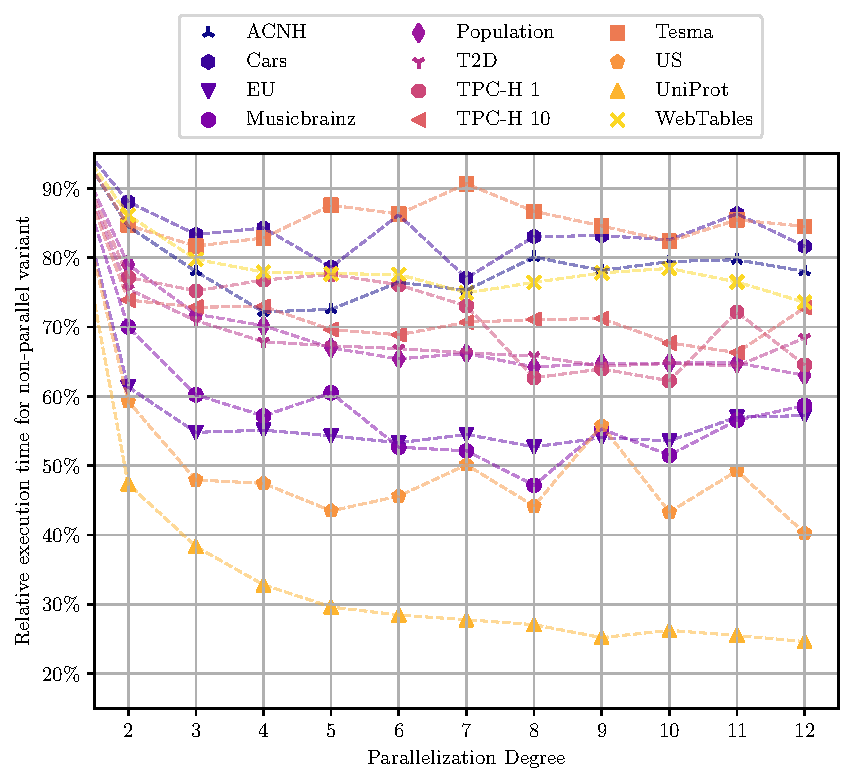
\includegraphics[width=0.475\textwidth]{figures/spider_parallel.pdf}
    \caption{Parallelization effectiveness for \textit{pSPIDER} over various datasets.}
    \label{fig:parallel_spider}
\end{figure}
\section{Parializing BINDER}
The \textit{BINDER} Algorithm \cite{papenbrock2015divide} is a IND discovery Algorithm which uses a divide and conquer technique to efficiently find unary and nary INDs. It was shown that \textit{BINDER} outperforms other exact, non-distributed state-of-the-art algorithms in both unary and nary settings \cite{dursch2019inclusion}. Due to its strong performance, this thesis offers a adapted version of \textit{BINDER} which can handle partial INDs, called \textit{pBINDER}.

\subsection{Existing Code}
The original \textit{BINDER} paper does not have a direct linkage to the source code used for the experiments. For the work conducted by Dürsch et al. on the comparison of multiple IND discovery algorithms\cite{dursch2019inclusion}, they published an implementation of \textit{BINDER} through GitHub\footnote{https://github.com/HPI-Information-Systems/inclusion-dependency-algorithms}. After talking to Thorsten Papenbrock, it turns out the source code found there is almost equal to the original code. The problem here lies within the poor structure of the code. Since a code base like this is neither readable nor well maintainable, the integration of partial constraints was a greater effort than initially expected. During the process of cleaning \textit{BINDER} I also bumped the needed dependencies to their most recent versions.

\subsection{Validator Adjustments}
The Validator of $BINDER$ handles the invalidation of IND candidates. Initially the algorithm assumes, that all candidates are valid. Whenever we find a conflicting value, meaning a value which is present in the depended side but not in the referenced side of a candidate, the validator removes the given candidate. To consider partial INDs we need to expand $BINDER$ such that the validator keeps track of the number of validations and only removes a candidate, if more validations than a given threshold have happened.

It is important to not that the partial $BINDER$ ($pBINDER$) implementation only supports a duplicate aware mode %TODO REF
. The concept and efficiency of $BINDER$ lies in the divide and conquer approach. The attributes are split into a set buckets using hash functions, such that the first bucket of each attribute maps the same subspace of values, e.g. there are $n$ buckets and we choses $hashCode \% n$ as the separation function. During the validation, the buckets are iterated in some order. At some point of the validation, we might already know, that the attribute is no longer included in any candidate. Loading the bucket now would be a waste of compute resources. There for we precisely skip these buckets. While this is great in a computational sense, $BINDER$ has no way of counting the number of distinct values, if not all buckets are loaded, especially if we would like to know the number of distinct values before the validation starts. Implementing duplicate unaware pIND discovery into $pBINDER$ would divert the algorithm too much from the original algorithm too a point where discussing the newly introduced complexity of pIND discovery would not make sense.



\begin{algorithm}
    \caption{Adjusted BINDER candidate pruning}\label{alg:BINDER_prune}
    \hspace*{\algorithmicindent} \textbf{Input:} value, valueGroup, pINDCandidates
    \begin{algorithmic}[1]
    \For{attribute in valueGroup}
        \State occurrences = attribute.getOccurrences(value)
        \For{candidate in pINDCandidates}
            \If{candidate.dependant $\not =$ attribute} 
                \State \textbf{continue}
            \EndIf
            \If{candidate.reference $\in$ valueGroup} 
                \State \textbf{continue}
            \EndIf
            \State candidate.violations += occurrences
            \If{candidate.violations $>$ candidate.maxViolations} 
                \State remove candidate
            \EndIf
        \EndFor
    \EndFor
    \end{algorithmic}
\end{algorithm}




% TODO test performance of rewrite and original


We will now discuss our proposed algorithm $SPIND$, which stands for \textbf{s}calable \textbf{p}artial \textbf{in}clusion \textbf{d}ependencies. Further the german word $Spind$ is a closet and often multiple "Spinds" are placed next to each other. This is a metaphor to the algorithms procedure. Every input relation will be transformed to a "Spind" of sorted values with connected attributes (attribute combinations), which is surely bigger than a $BINDER$ bucket, but there are far fewer "Spinds" than $BINDER$ would create buckets.

\subsection{Chunking the input relations}
Modern CPUs have multiple cores which can execute tasks in parallel. Most of the related work did not try to utilize multi-threading. $SPIND$ will multi-thread as many parts of the execution as possible to best utilize the available hardware. This goal requires us to find independent tasks which can be processes independent of each other. \\

\noindent The execution starts by fetching some very basic information about the input relations. For each relational instance (input table) $SPIND$ will extract the header column (if present) and store the number of columns each table has. Using a constant set by the user, $CHUNK_SIZE$, we spilt each relation into somewhat equal parts. Each chunk will consist of at most $\lfloor \frac{CHUNK_SIZE}{# cloumns \: in \: relation} \rfloor$ rows. The complexity of processing a relation directly depends on the number of total values in that relation. While this may be an oversimplification since there are many more factors, like the distribution of duplicate values, the raw size is easy to modify and a heuristic that can be applied without any specific dataset knowledge. Each of the resulting chunks is associated with exactly one relation and carries a subset of that relations rows. \\

\noindent Chunking is done exactly once at the very start and is not repeated for n-ary layers. We reuse the same chunks in every layer of the n-ary pIND discovery. \\

\noindent Since $SPIND$ almost always operates on the relation layer, a hash based partitioning, similar to $BINDER$, is not feasible. For the validation, we need to descend to the attribute layer and there we need to know which attributes share which values. If we partition the rows using a hash function, we could never guarantee some separation for every attribute (combination) without descending to the attribute layer already and therefore facing the same issues as $BINDER$.

\subsection{Sorting Chunks}
Once the chunks are created we want to sort each of them. Sorting is needed for the later validation.

\subsection{Merging (spilled) Chunks}

\subsection{Validation}

- shown in foundations that lower levels must be valid
- in that sense equal to INDs
- proposed generation of BINDER paper
- what are equal (p)IND representations
 - formal attribute and entry permutation
- prove the generation method

\subsection{Hyperparameter Optimization}
There are five hyperparameters which influence the execution of \textit{SPIND}. The size of the initially created chunks (\textit{CHUNK}), the maximal number of values which are kept in main memory during the sorting phase per thread (\textit{SORT}), the maximal number of files which are merged at once per thread (\textit{MERGE}), the queue size for each relation during candidate validation (\textit{VALIDATION}) and the degree of parallelization (\textit{PARALLEL}). Leveraging Bayesian optimization \cite{shahriari2015taking}, we seek to efficiently and iteratively identify parameter configurations that minimize the execution time of \textit{SPIND} of various datasets. We lower bound \textit{CHUNK} by 10,000 to avoid the creation of a massive amount of files and set an upper bound of 100 million. We limit \textit{SORT} between 10,000 and 3.5 million to find a balance between a large number of files being written and a safe number under the main memory threshold. \textit{MERGE} is lower bounded by two and upper bounded by 1,000 to not put too much pressure on the file system. \textit{VALIDATION} is upper bounded by 1 million. Finlay, \textit{PARALLEL} is upper bounded by the number of virtual threads of the executing machine.

A first observation is that \textit{PARALLEL} has a clear negative correlation with the execution time. Regardless of how the other four parameters are set. Figure \ref{fig:parallelization_effectivness} shows a group of hex-bin plots, where the y-Axis is always the degree of parallelization and the x-Axis take on the other variables. After X?X iterations, our estimated multi-variable function has a maximal $2\sigma$ uncertainty of X?X. These observations lead to the decision of fixing \textit{PARALLEL} to its upper bound.

The next iteration yields that \textit{CHUNK} is the second most important variable. While smaller chunks strictly correlate with the total number of files being created and therefore also the I/O overhead, we find an optimum at a chunk size of five million which is robust over different datasets. A smaller chunk size enables more tasks to be processed in parallel which has been shown to overcome the I/O operations at some point.

Summarizing the last three iterations, we find that \textit{SORT} and \textit{VALIDATION} should be as large as possible under the given main memory constraints. The results for \textit{MERGE} X?X %TODO

In Figure \ref{fig:chunk_size} we can observe the relative change in the number of files created under changing chunk sizes (left) and the relative execution times compared to the longest run (right). For these experiments, we always average the execution of three runs.

\begin{figure}
    \centering
    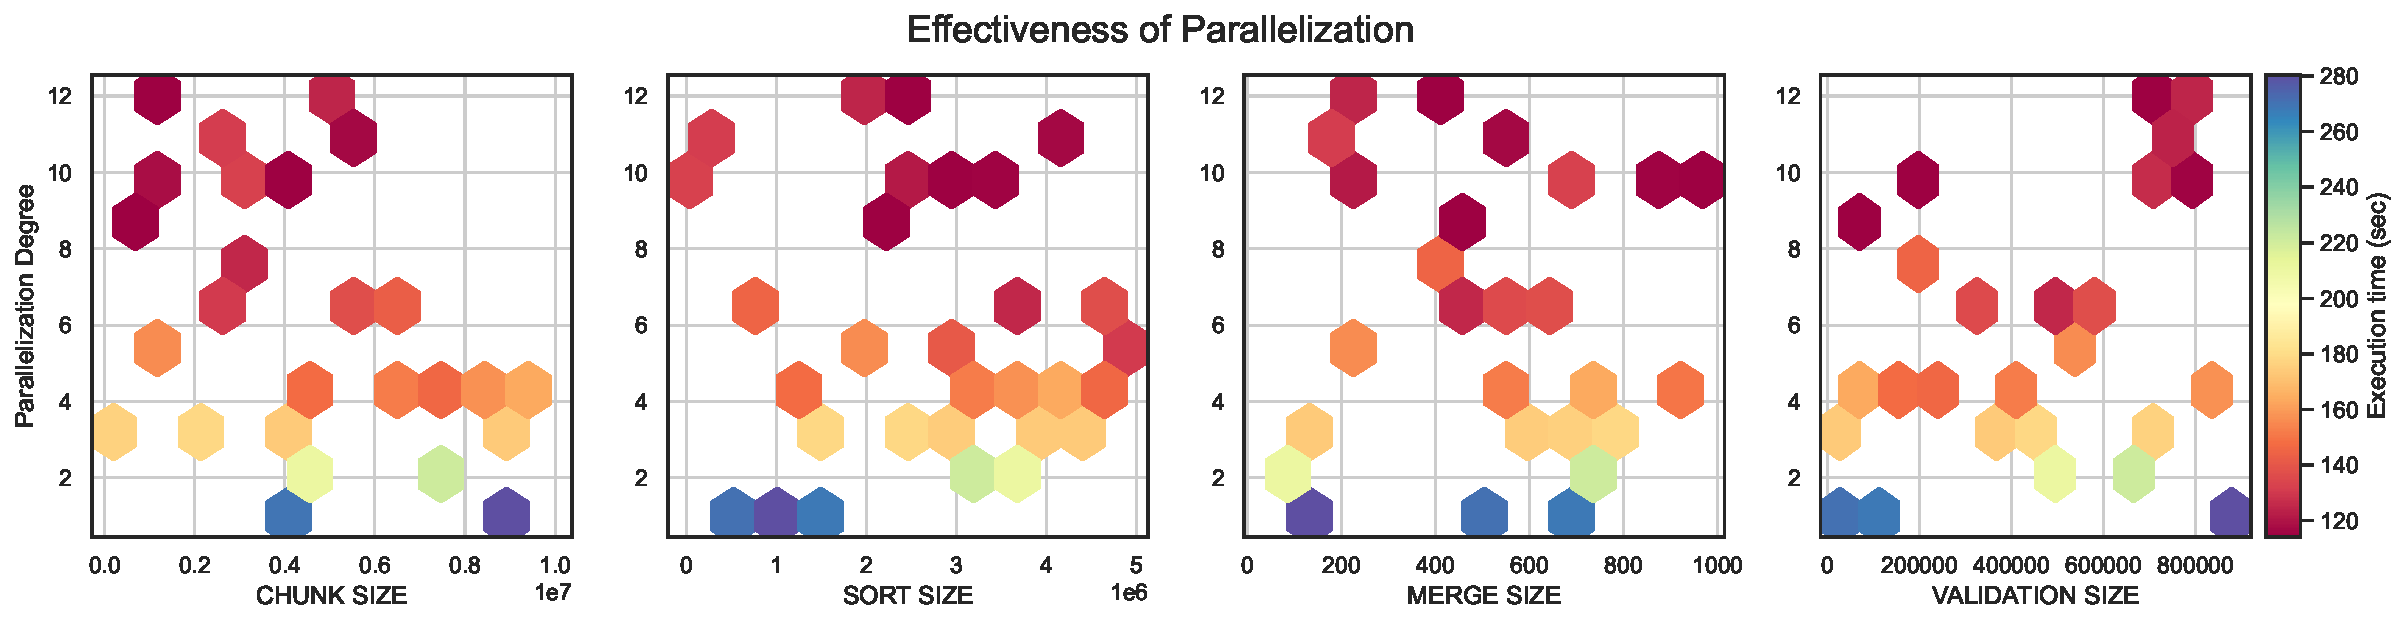
\includegraphics[width=.47\textwidth]{figures/parallelization.pdf}
    \caption{Effectiveness of the parallelization degree regardless of any other parameter.}
    \label{fig:parallelization_effectivness}
\end{figure}

\begin{figure}
    \centering
    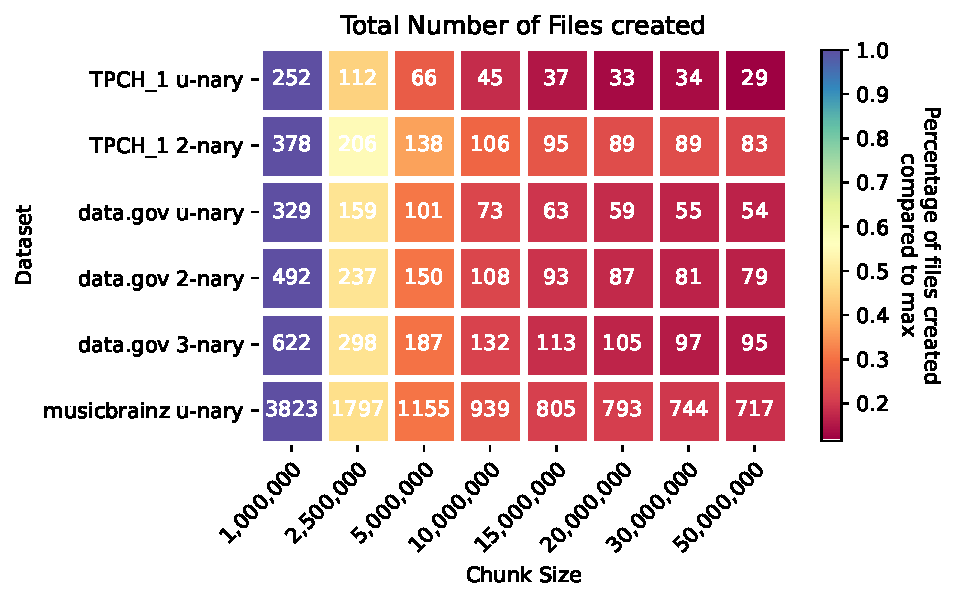
\includegraphics[width=.47\textwidth]{figures/chunk_size_files_created.pdf}
    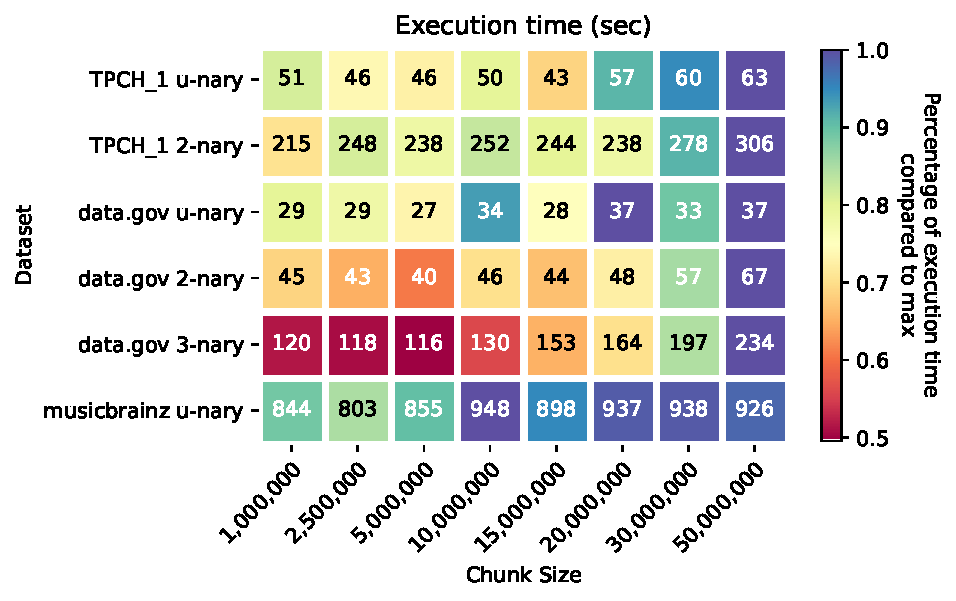
\includegraphics[width=.47\textwidth]{figures/chunk_size_execution_time.pdf}
    \caption{Files created (top) and execution time (bottom) under varying chunk sizes. Both relative to the maximum.}
    \label{fig:chunk_size}
\end{figure}

\section{Experimental Evaluation}\label{sec:eval}
To understand the practical performance of the proposed algorithms \textit{pSPIDER}, \textit{pBINDER} and \textit{SPIND} we use the known algorithms \textit{SPIDER} and \textit{BINDER} with their existing implementations. We will review the data sets utilized (Section \ref{subsec:datasets}) and present the execution times for all data sets across the different algorithms (Section \ref{subsec:runtime}). We will also discuss the impact of hyperparameter choices (Section \ref{subsec:hyperparameters}), the probabilistic filter (Section \ref{subsec:filter_res}), and finally examine pINDs in real-world data (Section \ref{subsec:real_pINDs}).

\chapter{Datasets}
To understand the performance of the proposed algorithms it is crucial to perform testing on a variety of data sets. For this purpose we will gather some real word data sets. Further we will create synthetic data sets that aim on edge cases to see if the performance is strongly dependent on structural assumptions.

\section{Real World Data Sets}
There are many sources for csv or tsv files online. I have decided to gather data from the US Government\footnote{\href{https://data.gov}{data.gov}}, the European Union\footnote{\href{https://data.europe.eu}{data.europe.eu}}, Kaggle\footnote{\href{https://kaggle.com}{Kaggle.com}}, Musicbrainz\footnote{\href{https://musicbrainz.org/}{musicbrainz.org}}, and Eurostat\footnote{\href{https://musicbrainz.org/}{ec.europa.eu}}. Further data set sources may be added. Related research papers sometimes discuss the origin of the used data, do not discuss the structure of the data they use \cite{papenbrock2017data,bauckmann2006efficiently, dursch2019inclusion, rostin2009machine}. In order to understand the resulting algorithm performance, we believe it is crucial to examine the data which is tested against. In this section we will discuss the data used and later try to understand why an algorithms performance may vary over different test sets.

\section{Synthetic Data Sets}
To evaluate the proposed algorithms under detailed aspects, we will generate synthetic data sets. The strategies and claims are based on \cite{jordon2022synthetic} synthetic data can be defined as \textit{data that has been generated using a purpose-built mathematical model or algorithm, with the aim of solving a (set of) data science task(s).} While we will not try to train a model with the synthetic data, it is still of great use for us, since we have absolute knowledge about the underlying structures. The decision is based on the fact that there is a lot of real word data available, since open data is a growing market which expected to grow even further \cite{EUopenData}. Synthetic data on the other hand enables us to evaluate the algorithm performances on edge cases, which we may not be able to find in the selection of real world data sets. \\

\noindent To test certain edge cases of the proposed algorithms, we will construct various edge case data sets. The \textit{SameSame} dataset consists of 32 attributes and 250.000 records. Each attribute carries the numbers 1 to 250.000 in the natural order. This means every attribute is a (partial) inclusion dependency of every other attribute. The same obviously also holds for combinations of columns. We will now calculate the expected number if (p)INDs in each layer. Since all candidates are perfect matches, the chosen threshold $\rho$ will not influence the number of pINDs. Table % TODO add ref
shows the number of candidates/pINDs for the \textit{SameSame} dateset.
% TODO calculate INDs
The edge case to test here is, how well the algorithm can understand equality relations and prune the candidate space. While this may seem like an unlikely edge case we will also investigate how often this happens in real world data sets. \\
% write about real world structures

\noindent Another source of synthetic data will be the TPC (Transaction Processing Performance Council) Benchmarks \footnote{\href{https://www.tpc.org/}{tpc.org}}. The TPC Benchmarks are a set of standardized and vendor-neutral performance benchmarks used to evaluate the processing and database capabilities of different systems. These benchmarks are designed to model various types of workloads. The TPC-E benchmark, for example, models a brokerage firm with customers who generate transactions related to trades, account inquiries, and market research, while the TPC-C benchmark is intended to model a medium complexity online transaction processing workload, patterned after an order-entry system with skewed access within individual data types/relations. Using scaling factors, a user can define the size of the synthetic database themselves. This enables us to examine the algorithm performances in a very controllable setting.



\subsection{Filter Evaluation} \label{subsec:filter_res}
We would like to understand the effect of using a probabilistic filter. In Section \ref{subsec:prob_filter} we discuss two versions. A filter which is built once after unary discovery and a filter which is rebuild on every nary layer. In Figure \ref{fig:filter} we find the execution times of all datasets, expect \textbf{WebTables} since we only search for unarys in that case. The graphic shows the difference in runtime when using the bloom filter by constructing it once during unary discovery (\textit{Once}), using and refining the filter at every level (\textit{Refine}) and not using a probabilistic filter at all. Not using a filter builds the baseline execution time, while the other two modes are displayed with their relative runtime to that baseline.

We find that the results vary substantially when viewing the different datasets. This observation supports the notion that we succeeded in finding a range of datasets which are structurally different from each other. Notably, \textit{TPC-H 1} and \textit{UniProt} performed better without a probabilistic filter. For \textit{UniProt} we find that the filter does decrease the execution time since the data set exclusively produces symmetrically INDs. For \textit{TPC-H 1}, we observe that the number of n-ary candidates is so limited that the time spent on construction exceeds the computational savings achieved. Employing either a filter build once or a refined filter yields nearly identical execution times, which are generally slightly quicker than not using a filter at all. Given that a refined filter can reduce some read and write operations, we opt for this version to reduce the disk workload.

\begin{figure}[t!]
    \centering
    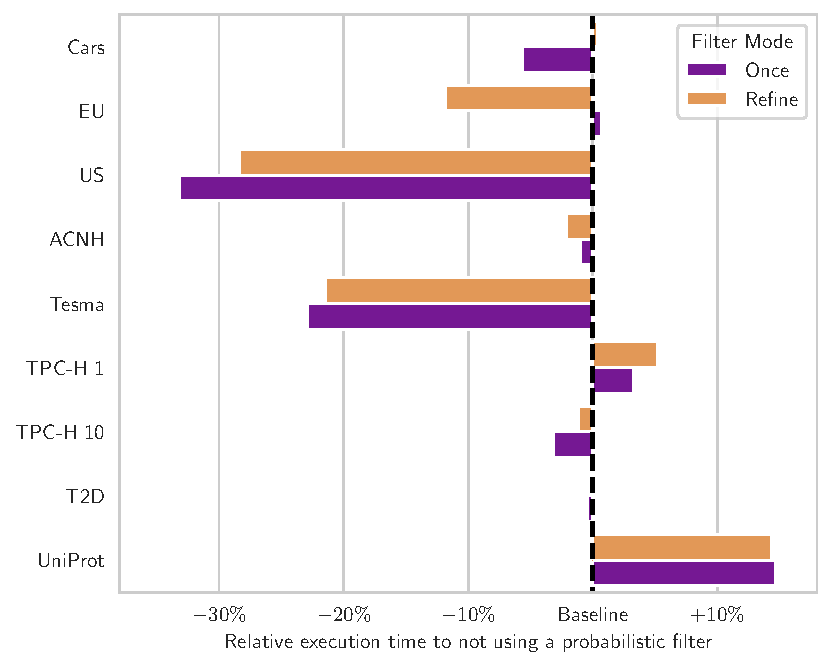
\includegraphics[width=.48\textwidth]{figures/filter_results.pdf}
    \caption{Changes in execution time when using a (refined) probabilistic filter for nary IND discovery.}
    \label{fig:filter}
\end{figure}

\subsection{Real World pINDs} \label{subsec:real_pINDs}
Real-world datasets exhibit a considerable amount of pINDs, even when the identification threshold for such relationships is set to a high value (e.g., $\rho = 0.99$). Some of these pINDs are logical and significant, indicating underlying patterns or connections within the data. For example, date columns may not be perfectly contained within each other due to differences in update frequencies across data sets (found in the \textit{EU} data set). However, pINDs also occur purely by chance, without any substantial relevance. Consequently, human expertise is essential to evaluate whether a discovered pIND is truly useful, as automated detection alone cannot adequately distinguish between meaningful dependencies and coincidental ones.

% This document should discuss passed approaches focusing on pros and cons

\section{Related Work}\label{sec:rel_work}

Inclusion dependencies (INDs) are a highly influential concept in both database research and practice, with a wide range of contributions and applications. The introduction already provided some insight into their diverse application areas of INDs. In this section, we will focus on the key achievements related to the implication problem of INDs. We will go over different algorithms and discuss their unique features. \\

In 1981 INDs started as a general notation of referential integrity, which was already a well established concept back then \cite{date1981referential}. Casanova et al. presented a paper on the inference rules of INDs\cite{casanova1982inclusion}. Three axioms where introduced: \textit{reflexivity}, \textit{transitivity} and \textit{projection and permutation}. The application of these rules to partial INDs will later be discussed in detail (Section \ref{theo:pInd}). The paper further proofed that the discovery of INDs is PSPACE-complete if there is no limit on the size of inclusions. Publications typically fall into three groups of algorithms, foreign key discovery algorithms, unary IND discovery and n-nary IND discovery \cite{papenbrock2017data}. \\

In 1995 Bell and Brockhausen \cite{bell1995discovery} propose a graph-based approach to represent the relationships between attributes, allowing for a more efficient exploration of the search space. The algorithm is initiated with a directed graph, wherein all possible edges, which could not be pruned by statistical measures, are included. A directed edge in the graph represents an inclusion dependency, which is read as the edge from $A_i$ to $A_j$ ($A_i \rightarrow A_j$) represents the IND $A_i \subseteq A_j$. It then proceeds to remove those edges that failed the IND check. To determine the validity of an edge, the algorithm checks for transitivity, which enables it to answer whether a dependency could exist between two variables based on their relationships with a third variable, which was tested previously. If it is ascertained that a dependency is impossible, the algorithm skips the test and directly removes the given edge, thereby reducing the overall computational cost. The approach presented by Bell and Brockhausen for unary IND discovery has both reusable aspects and downsides. The algorithm's candidate generation technique, which uses data statistics such as data types and min-max values, can be reused in other discovery algorithms. This preprocessing step reduces the number of candidates that need to be validated and further reduce the storage overhead needed to store candidates. However, the validation technique used in the algorithm, which relies on SQL join-statements and requires accessing the data on disk, is infeasible for larger candidate sets. This limits the scalability of the approach and makes it less practical for large-scale data sets. Additionally, the need to store the data in a database and access it on disk for validation can add to the computational cost and time required for the discovery process.\\

The \textit{SPIDER} algorithm is a disk-backed, all-column sort-merge join with early termination used for the discovery of inclusion dependencies \cite{bauckmann2006efficiently}. It sorts the values of each attribute, removes duplicate values, and writes the results to disk in the first phase. In the second phase, it performs the actual inclusion dependency discovery by using a pointer for each file and validating all candidates at the same time. A major advantage is, that in this setting every value only needs to be read a single time from disk, which greatly reduces the I/O bottleneck. The Spider algorithm has been the subject of experimental evaluation and is considered one of the efficient techniques for unary IND discovery. Still, there are drawback if the data set is too big to be sorted in main memory or if the number of simultaneously open files allowed by the OS system is reached \cite{papenbrock2015divide}. \\

In 2009 Bauckmann et al. also proposed a partialized version of $SPIDER$ in a section of the same paper. The authors found that there where surprisingly many partial inclusions (under a 5\% threshold) in their test data sets. To find partial inclusion dependencies, they first count how many distinct violations are present and in a second step consider the amount of duplicates for not included values. This means their algorithm does not immediately stop once a single validation has been found but only after an added counter surpasses a given threshold. The paper is not particular clear on how the number of duplicates is stored/retrieved and additionally does not analyse the computational effect of these changes and with the original source code being lost, this a approach can only be verified using a best guess approach.\\

The \textit{SAWFISH} algorithm \cite{kaminsky2023discovering}, published in 2023, is designed for identifying similarity inclusion dependencies (sINDs) within datasets, introducing a novel perspective on inclusion dependencies (INDs). While traditional INDs assume error-free data, \textit{SAWFISH} incorporates a similarity measure to accommodate minor errors like typos. Given a similarity threshold $\omega$ a sIND is valid if and only if for all tuples in the left hand side there exists a tuple in the right hand side which has at least a similarity of $\omega$ under a set similarity measure. The authors used the edit distance as well as the normalized edit distance. Through preprocessing, metadata generation, and a sliding-window approach, \textit{SAWFISH} successfully identifies and validates sIND candidates using an inverted index, providing a valuable tool for database applications despite dirty data challenges. \\



\section{Future Work}
We are aware that there is still potential left to improve pIND discovery. A central observation in the complex datasets with large n-ary pINDs is, that the generated candidates eventually become equal or almost equal to the valid pINDs of some layer. An idea would be to jump a few layers ahead if such a thing happens since it strongly hint towards the existence of pINDs in a (much) deeper layer. In \textbf{ACNH} we find that from the sevens to the twelves layer the generated candidates where always all valid.

The published code behind the algorithm can also be improved further. The implementation mostly relies on standard java data structures. There are libraries, such as FastUtil\footnote{\url{https://fastutil.di.unimi.it/}}, which offer high performance versions of these structures and may be able to improve the performance. Serialization is also performed in a human-readable style, which is not optimal. Encoding the attribute ids and occurrences (integers and longs) in one and four byte blocks could decrease the file size drastically which could help when I/O bottlenecks occur.

%%% End of paper content %%%

%\clearpage

\bibliographystyle{ACM-Reference-Format}
\bibliography{sample}

\end{document}
\endinput
